\documentclass[11pt,a4paper]{article}
\usepackage{tikz}
\usetikzlibrary{arrows.meta,positioning}
\usepackage{tabularx}
\usepackage{amsmath,amssymb,amsthm}
\usepackage{geometry}
\geometry{margin=1in}
\usepackage{hyperref}
\usepackage{graphicx}
\usepackage{setspace}
\onehalfspacing

\title{\textbf{Paper G-01: Language Evolution:\\ A Constraint-Driven Flux Dynamics (CDFD) Perspective}}
\author{Steve Bico Mujjabi, MD\\
\small Independent Researcher\\
\small Founder, Vura Labs\\
\small Kampala, Uganda\\
\small ORCID: 0009-0001-0556-5516}
\date{August 2026}

\begin{document}
\maketitle

% BEGIN SHARED-METHODS POINTER
\noindent\textit{Shared Part IV notation and evidence boundaries are defined in \path{PART_IV_METHODS_AND_CLAIM_BOUNDARY.md}. This paper states only its local observables, comparison, and failure conditions.}
% END SHARED-METHODS POINTER


\begin{abstract}
This paper develops a falsifiable CDFD/AFL model of Language Evolution. It maps utterances, meanings, learners, media, and social interaction to driving flux $\Phi$, cognition, channel capacity, social structure, ambiguity, and convention to active constraint $C$, innovation, repair, learning, borrowing, and accommodation to responsiveness $S$, and grammar, lexicon, corpora, identity, institutions, and historical contact to structural memory $M_s$. The target outcome is intelligibility, change, diffusion, and linguistic diversity, tested against corpora, experiments, social networks, historical records, and longitudinal language data. The paper treats universality as a shared model architecture rather than an assertion that unlike systems have the same material mechanism. It states the negative result that would make the mapping unnecessary and places the domain claim inside the cumulative CDFD programme and its reproducible runtime boundary.
\end{abstract}

\section{Introduction}

Language is not a static repository of symbols; it is an active, self-regulating biological and social phenomenon. Words are invented, adopted, mutated, and discarded at rates that mirror genetic drift and viral epidemiology.

When a language spreads across a wide geographic and social space, changing contact networks can limit communication and support dialect formation. CDFD treats this as a testable interaction among information flow, network constraint, adaptive repair, and historical memory rather than an inevitable breakdown.

\section{Linguistics as an Adaptive Surface}
We apply the Adaptive Operating Ratio to the domain of human communication:
\begin{equation}
    \Psi_s = \left( \frac{\Phi}{C} \right) \cdot S \cdot M_s
\end{equation}

For a language group, the parameters map directly to informational transport:
\begin{itemize}
    \item \textbf{Flux ($\Phi$)}: The daily volume of communication, trade, and memetic exchange occurring across the population.
    \item \textbf{Constraint ($C$)}: Geographic boundaries (mountains, oceans), political borders, or simply the physical limits of ancient communication speeds.
    \item \textbf{Responsiveness ($S$)}: The cognitive plasticity of the population, particularly the youth, who act as the primary agents of linguistic innovation and adoption.
    \item \textbf{Memory ($M_s$)}: The formal grammar, written records, and academic institutions that standardize the language. High memory rigidly enforces "correct" usage, resisting phonetic drift.
\end{itemize}

\subsection{Dialectic Bifurcation and Regime Shifts}
Consider a unified language spoken across an expanding empire. Initially, trade and travel are high ($\Phi$ is large), maintaining a healthy communicative regime ($\Psi_s \approx 1$).

If the empire fractures, the constraint ($C$) between two provinces drastically increases. The cross-border flux $\Phi$ drops. Consequently, the adaptive ratio across that specific geographical border plummets to $\Psi_s \ll 1$. The system is in "communicative decay."

To restore local equilibrium, the isolated nodes (provinces) must adapt internally. Cut off from the central normalizing flux, their local youth populations (high $S$) begin optimizing the language for local efficiency, introducing slang and phonetic shifts. The central, formal grammar (high $M_s$) can no longer suppress these changes because the regulatory flux ($\Phi$) from the capital is gone. The language bifurcates. What was once a unified active surface topologically splits into two distinct, localized surfaces, each achieving its own stable $\Psi_s \approx 1$ state as a new, distinct language (e.g., the fracturing of Latin into the Romance languages).



\section{Measurement Layer}

% BEGIN PART IV MAJOR CROSS-DOMAIN UPGRADE
\section{Cross-Domain Model Upgrade: Mechanism, Scale, and Tests}

\subsection{Observable Translation}

The paper-specific translation begins with an observable chain rather than a
verbal analogy. For Language Evolution, the proposed drive is utterances, meanings, learners, media, and social interaction.
The active limitation is cognition, channel capacity, social structure, ambiguity, and convention. Responsiveness is carried by
innovation, repair, learning, borrowing, and accommodation, while retained state is represented by
grammar, lexicon, corpora, identity, institutions, and historical contact. The outcome to explain is intelligibility, change, diffusion, and linguistic diversity.

\begin{table}[htbp]
\centering
\small
\caption{Operational CDFD/AFL map for Paper G-01.}
\begin{tabularx}{\textwidth}{|l|X|X|}
\hline
\textbf{Term} & \textbf{Paper-specific observable meaning} & \textbf{Measurement question} \\
\hline
$\Phi$ & utterances, meanings, learners, media, and social interaction & What rate, load, gradient, or demand enters the focal system? \\
\hline
$C$ & cognition, channel capacity, social structure, ambiguity, and convention & Which measured bottleneck limits transfer, function, or recovery? \\
\hline
$S$ & innovation, repair, learning, borrowing, and accommodation & Which process changes effective capacity or reroutes the load? \\
\hline
$M_s$ & grammar, lexicon, corpora, identity, institutions, and historical contact & Which retained state makes equal present loads produce different futures? \\
\hline
$Y$ & intelligibility, change, diffusion, and linguistic diversity & Which outcome is predicted out of sample, with uncertainty? \\
\hline
\end{tabularx}
\end{table}

\begin{figure}[htbp]
\centering
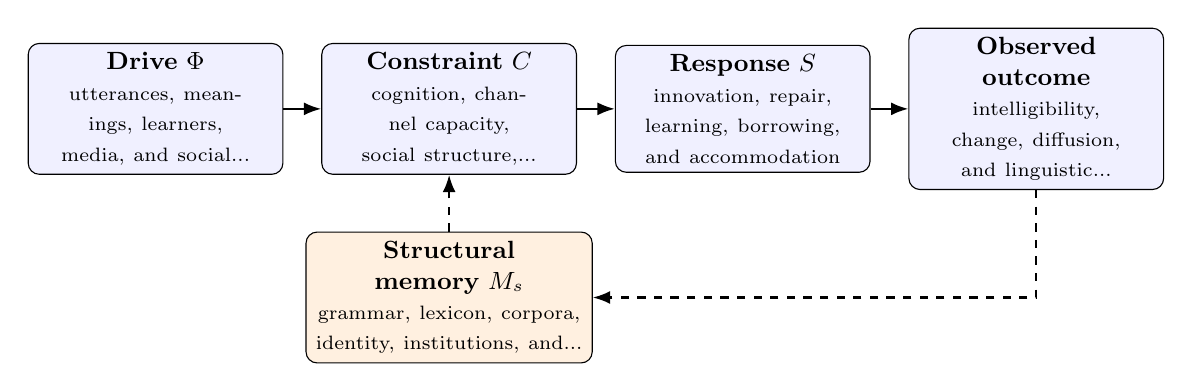
\begin{tikzpicture}[
    node distance=0.48cm,
    every node/.style={font=\small},
    box/.style={draw, rounded corners, align=center, minimum height=1.45cm, text width=3.0cm, fill=blue!6},
    memory/.style={draw, rounded corners, align=center, minimum height=1.25cm, text width=3.4cm, fill=orange!12},
    flow/.style={-{Latex[length=2.2mm]}, thick},
    feedback/.style={-{Latex[length=2.2mm]}, thick, dashed}
]
\node[box] (drive) {\textbf{Drive $\Phi$}\\\scriptsize utterances, meanings, learners, media, and social...};
\node[box, right=of drive] (constraint) {\textbf{Constraint $C$}\\\scriptsize cognition, channel capacity, social structure,...};
\node[box, right=of constraint] (response) {\textbf{Response $S$}\\\scriptsize innovation, repair, learning, borrowing, and accommodation};
\node[box, right=of response] (outcome) {\textbf{Observed outcome}\\\scriptsize intelligibility, change, diffusion, and linguistic...};
\node[memory, below=0.72cm of constraint] (memory) {\textbf{Structural memory $M_s$}\\\scriptsize grammar, lexicon, corpora, identity, institutions, and...};
\draw[flow] (drive) -- (constraint);
\draw[flow] (constraint) -- (response);
\draw[flow] (response) -- (outcome);
\draw[feedback] (outcome.south) |- (memory.east);
\draw[feedback] (memory.north) -- (constraint.south);
\end{tikzpicture}
\caption{Paper G-01 observable CDFD/AFL architecture for Language Evolution. Solid arrows give the proposed forward chain; dashed arrows make history-dependent feedback explicit.}
\label{fig:g01-architecture}
\end{figure}

\subsection{Paper-Specific Causal Hypothesis}

For this paper, the hypothesized causal sequence is specific. A change in
utterances, meanings, learners, media, and social interaction arrives faster than innovation, repair, learning, borrowing, and accommodation can compensate.
This raises or redistributes cognition, channel capacity, social structure, ambiguity, and convention. If the load persists,
the retained state encoded by grammar, lexicon, corpora, identity, institutions, and historical contact changes the next response, so a later event of equal
magnitude can produce a different trajectory in intelligibility, change, diffusion, and linguistic diversity. The
scientific task is to estimate that sequence against the best ordinary model of
the domain, not merely to redescribe the outcome after it occurs.

\subsection{Cross-Scale Translation Without Mechanistic Erasure}

For the abstract and cognitive systems family, the cross-domain translation compares information-bearing activity, limited channels or institutions, adaptive reorganization, and retained semantic or technical structure. Because meanings and goals are not conserved physical quantities, every mapping must state its observational unit and avoid treating metaphor as measurement. \cite{Shannon1948,BarabasiAlbert1999,WattsStrogatz1998,Turing1952,BakTangWiesenfeld1987}
The required scale declaration for this paper is milliseconds to millennia; speakers to language families. At short
scales, the key question is whether the incoming drive is transmitted,
buffered, or diverted. At intermediate scales, response changes effective
capacity and network exposure. At long scales, retained structure can alter the
state space itself. A result is genuinely cross-scale only when the aggregation
rule is stated and the same conclusion is not an artifact of averaging.

\subsection{Evidence Ladder and Discriminating Tests}

\begin{table}[htbp]
\centering
\small
\caption{Evidence ladder for Paper G-01. Each rung can fail independently.}
\begin{tabularx}{\textwidth}{|p{0.17\textwidth}|X|X|}
\hline
\textbf{Test} & \textbf{Design} & \textbf{Discriminating result} \\
\hline
Proxy audit & Measure corpora, experiments, social networks, historical records, and longitudinal language data and preregister how each record maps to $\Phi$, $C$, $S$, $M_s$, and $Y$. & The mapping fails if proxies are non-identifiable, circular, or change meaning across cases. \\
\hline
Load ramp & Apply or observe a communication or contact shift across communities with different histories while estimating the dominant constraint and response time. & A threshold claim requires a reproducible nonlinear change and uncertainty bounds, not a visually chosen breakpoint. \\
\hline
Recovery and memory & Match present load across units with different histories, then compare recovery paths. & The memory claim requires history-dependent divergence after current conditions are controlled. \\
\hline
Model comparison & Compare the baseline domain model with and without the CDFD/AFL state variables using held-out data. & The paper's stated falsifier is: constraint-memory terms do not improve language-change or comprehension prediction. \\
\hline
\end{tabularx}
\end{table}

\subsection{Research Programme and Boundary Conditions}

The immediate research programme has four steps. First, construct a documented
dataset from corpora, experiments, social networks, historical records, and longitudinal language data and retain raw units before normalization.
Second, fit a baseline domain model and report its calibration and out-of-sample
error. Third, add the smallest identifiable CDFD/AFL state extension and test
whether it improves prediction of intelligibility, change, diffusion, and linguistic diversity. Fourth, repeat the
analysis across the declared scale range and publish negative cases as part of
the cross-domain translation audit.

% END PART IV MAJOR CROSS-DOMAIN UPGRADE

\section{Conclusion}
Language evolution is not exempt from the laws of universal thermodynamics. Grammatical rules are systemic memory; communication is energetic flux; and dialects are structural bifurcations born of chronic constraint. CDFD suggests that information networks, whether composed of neurons, electrical grids, or human speech, optimize their topology using the same candidate mathematical structure.
\section*{Conflict of Interest} The author declares no conflict of interest.
\section*{Data Availability}
Part-specific runtime diagnostics are under each Part's \path{outputs/} directory.

Release-wide code: \path{Part_E_Synthesis/supplementary/}.

Generated summaries: \path{Part_E_Synthesis/outputs/}.

Figures: \path{Part_E_Synthesis/figures/}.


\section{Reference Layer}
\bibliographystyle{plain}
\bibliography{universal_afl_references}
\end{document}
